\documentclass[10pt,twocolumn,letterpaper]{article}

\usepackage{times}
\usepackage{epsfig}
\usepackage{graphicx}
\usepackage{amsmath}
\usepackage{amssymb}

% Include other packages here (if needed), before hyperref.

% If you comment hyperref and then uncomment it, you should delete
% egpaper.aux before re-running latex.  (Or just hit 'q' on the first latex
% run, let it finish, and you should be clear).
\usepackage[breaklinks=true,bookmarks=false]{hyperref}



%numbering the pages
\setcounter{page}{1} 
\begin{document}


%%%%%%%%%%%%%%%%%%%%%%%%%%%%%%%%%%%%%%%%%%%%%%%%%%%%%%%%%%%%%%%
% DO NOT EDIT ANYTHING ABOVE THIS LINE
% EXCEPT IF YOU LIKE TO USE ADDITIONAL PACKAGES
%%%%%%%%%%%%%%%%%%%%%%%%%%%%%%%%%%%%%%%%%%%%%%%%%%%%%%%%%%%%%%%



%%%%%%%%% TITLE
\title{Music Recommendation Systems CSC461 Project -  Final Report}

%update the number of authors and names and emails based on your group
\author{Miguel Ibrahim\\
{\tt\small miguel.ibrahim@lau.edu}
\and
Omar Majzoub\\
{\tt\small omar.majzoub01@lau.edu}
%\and
%Fourth Author\\
%{\tt\small fourthauthor@pu.edu.lb}
}

\maketitle
%\thispagestyle{empty}



% MAIN ARTICLE GOES BELOW
%%%%%%%%%%%%%%%%%%%%%%%%%%%%%%%%%%%%%%%%%%%%%%%%%%%%%%%%%%%%%%%

%%%%%%%%% ABSTRACT
\begin{abstract}

The idea behind the recommendation system is for companies to keep the users using the application for as long
as possible; however, this implication does not go hand
in hand when it comes to providing a bulk set of information that could be daunting to the user.
Therefore, this paper is dedicated towards creating model that recommends
one song at a time to listen to rather than a bulk of data presented in a playlist. This model
is similar to other models, but simplicity is taken into account, where previously listened-to songs are mainly considered. In this model, the data set that is being used
does not have enough features, and may not be enough
to create accurate output. \cite{pichl2015towards} After adding a genre feature
in place of the playlist name column hoping to create a
much more specific output than the data set can provide.
Previous research on this model is related to recommender systems, and it is capable of creating a custom recommender system without complicating it too much by not requiring many features. In this case, three different approaches were used stemming from the
same LightFM model. Each had a focus on other features that may help increase AUC and precision. The first method considers how frequently songs were listened to and uses pure collaborative filtering (CF). The results are AUC: (train: 0.9716839, test: 0.97279567),
and Precision@K (k=5): (train: 0.40, test: 0.22). The
second method does not use frequency. The hybrid (CF
and content-based filtering) model gave the following results: AUC: (train: 0.976131, test: 0.9232743), and Precision@K (k=5): (train: 0.388438, test: 0.06182772).
The pure CF model gives AUC: (train: 0.99326223, test: 0.9158364), and Precision@K (k=5): (train: 0.6124809,
test: 0.044162657).

\end{abstract}

%%%%%%%%% BODY TEXT
\section{Introduction}
As mobile applications have made digital music much more available than before, it would take much time and effort to sort such data. As a result, automating the process of searching through music libraries and recommending songs that users might like by creating a music recommender system can be greatly beneficial. \cite{ADIYANSJAH201999} In this project, there is an attempt to build a music recommender system hoping to help solve this issue.

To begin with, the data set available on the Jupyter Notebook and Google Colab has gathered users' data using the Kaggle Spotify playlist \cite{larxel_2021}. This data set gathers users' data to recommend them a set amount of artists that are close to his/her frequently listened-to artists. The data set is what is used to allocate a recommended playlist every week to a specific user based on his/her frequently listened-to songs, liked songs and cosine similarities, or k-means to other similar songs. In the case of LightFm however, it recommends a song based on the interaction matrix, where if user A and B listen to the same songs, but, user B listens to one more song, user A will be recommended the song from user B.

There exist many different ways to recommend a song, two of the most notable ones are of Content-Based Filtering and Collaborative Filtering. The Similarities in the features user have and/or items are used in Content-Based filtering to make recommendations, whereas pure Collaborative filtering only uses the interactions between users and items to find similarities and ultimately create a recommendation for the user. \cite{mingzhi_2021} In the case of the model being presented in this paper, it consists of a LightFM model, a deep learning model, that can be purely Collaborative or a hybrid of Collaborative Filtering and Content-Based Filtering models and approaches. \cite{mingzhi_2021}


To explain Content-Based filtering one needs to give an example. Let's say user\_1 bought a ladder with a paint bucket, the model will try to understand the intentions of this user and classify them as wanting to paint a wall. Similar users that want to buy a paint bucket will be recommended a ladder since the last user bought them together. 

Data prepossessing was performed at the beginning of this project. Understanding the data set took some time to go through and reach a conclusion. It, therefore, turns out to be a collection of user data in their own created playlists. The similarity presented in the user\_id and playlist name gave it away, but the different artist names made it obvious that it is a collection of the user's data rather than the artist's data. However, there exists a column in the data set that is not necessarily important for the precision of the data set - the user's playlist name. It is theorized that it isn't going to help much in creating a clustering model for the system, furthermore, it creates an overhead to the computational cost considering the 12.8 million rows, and it may cause the model to infer similarities that do not make much sense possibly resulting in unwanted relations between different aspects.

However, it is theorized that the playlist plays a role in creating a clustering model in a form of a circle where each user has his/her own cluster where if a new user is created and has similar features, then they will be recommended some songs from the other person. There exists a huge sum of data in the Spotify data set. This serves to show how technology has evolved through the years and how it became hard to recommend a song to a specific person based on his/her taste. This proves that ML has helped a great deal when it comes to recommending songs to users rather than manually doing it, which is a good thing in today's world since ML is becoming accurate and efficient. 

After uploading the CSV file to Jupyter Notebook and saving the data into a data frame to begin processing it by dropping similar rows, null values, and Unnamed rows such as the row numbers usually created after loading a data set. Furthermore, a genre column is added instead of the playlist name using The University of Waterloo's data set \cite{tompkins_n.d.}. Web scraping was performed in order to match songs to the respective genres. Not all songs matched and our data set was reduced to about 150,000 rows. This method is used to increase the likelihood of getting accurate results such as the artist's name and the music to listen to from that artist. The reason behind that is that one artist can have different genres of music, recommending the artist alone is not a good idea because it would not cut down on the choices that Spotify provides. Furthermore, it would add an unnecessary element to the steps to be taken to listen to a song, which is browsing through the artist's contents and manually choosing a song that the user likes or wants to try out. The original plan was to create a music recommender system that funnels down the choices to an output that looks like: "We recommend:1. Aria by C418 Genre: calming" rather than: "1. C418 2. Lena Raine." (C418 and Lena Raine are artist names).

\section{Related Work}
One of the most significant related works is Spotify and Anghami itself, the music recommendation model is one of the most popular types of machine
learning model these days. There exist multiple related works on this topic, some use many different types of ways to recommend music, and there does not exist
a specific algorithm for music recommendation systems. The closest related work to the current project is the personalized music recommender system by Galety
et al.(2022) \cite{09782288}. This recommender system uses cosine similarity and a count vectorizer to use the information gathered from user evaluations that are used to make suggestions for the user. The model being created is somewhat close to the model that is presented
by Galety et al.; however, it differs in how the output
is displayed. Rather than the output being displayed
as a playlist containing the recommended songs, 
the model being worked on in this paper will recommend one song at a time for more
ease of use and user experience considering the lack
of time users have these days due to their focus on
jobs, family, and more important matters rather than
spending their time nitpicking the best song from the
playlist provided to them. There exist many other
music recommendation systems that use different algorithms such as LightFM, k means, and non-machine learning algorithms such as the If-Then algorithm (which is not an algorithm).

In the research paper behind the data set that was used,
Pichl et al. \cite{pichl2015towards} performed clustering based on the
playlist names by using NLP and tried to build a music recommender system based on the context that the
playlist names would indicate. Their work resulted in
an increase in accuracy by 33\% of ”collaborative filtering recommender systems” \cite{pichl2015towards}. The authors of this paper hope to obtain better accuracy by using genres instead of playlist names in the dataset.


\section{Proposed Method}
The proposed method to be used on the Kaggle dataset is a well-known recommender system called LightFM. According to the documentation presented by Kula(2016)\cite{kula_2016}, it is a popular recommender algorithm that "represents each user and item as the sum of the latent representations of their features, thus allowing recommendations to generalize to new items (via item features) and to new users (via user features)."

After that, it was necessary to fit LightFM into a model that can be used for the data set, one of them stemmed from a Kaggle coder called Pegah Pooya\cite{pooya_2021}. Their method is a pure CF LightFM model that only takes user\_id and artist name into account, and it took into consideration the frequency of the artists of the songs that were listened to. This method was taken and adjusted to take into account the tracks instead of the artist names and their frequency. Recommending an artist is not something this paper wanted to achieve as mentioned above, recommending a song title reduces the effort being put in by the user to search for his/her favorite song in the artist's dictionary of songs.
The authors will proceed to call this method "Method 1". 

On the other hand, methods two and three codes were mainly written by Sha on GitHub Pages \cite{mingzhi_2021} to demonstrate how to configure a data set for LightFM and then create both a pure LightFM and a hybrid model that takes into account the item features in the data set such as the genre column in our case. This method was taken and adjusted to our data set where instead of the products in Sha's code, tracks were used and a random state parameter was set (=42) to obtain consistent results in the final model. Other parameters were left the same as Sha's code in the final notebook. A new column for track\_id was made by using the labelEncoder function from scikit-learn to have a column similar to Sha's product\_id. As a result of this code, two models have been obtained: a pure CF model taking into consideration the user\_id and track id, and a hybrid model combining CF and content-based filtering using the artist, track (track name), and genre as features of the tracks. These methods will be called "Method 2" and "Method 3" respectively. Track features were standardized by LightFM in Method 3.

\section{Experiments}

Before using the three different models for the data set, a lot of research has been done on how to exactly create a music recommender system; their research provided only theoretical ideas rather than the code they worked on. This did not help much in further understanding how the code interacts with the data set. With further research, and searching, Kaggle's wide variety of coders presented a unique and custom-made code that uses the data set that was downloaded from Kaggle itself. After that, a similar model was found via extensive browsing which led the authors to fixate on the three different methods on the two mentioned websites (Kaggle Notebook by Pooya and Sha's article).

As for the experiments, the data set was not the exact same as it was after downloading it directly from Kaggle, it was reduced significantly after web scraping and referencing the results with the dataset extracted from the University of Waterloo \cite{tompkins_n.d.} to add the genre column and replace the playlist name column. The recommended results were listened to by one of the authors in this paper to assess if the recommended songs are somewhat accurate or not. In this case, the author tried ten different users, which all got recommended other songs, and all passed the auditory testing. However, the experiments were done with a user that does not listen to the songs, so it was necessary to create a custom curated user\_id with their own songs they listen to. Miguel inserted his own songs he listens to daily, at least more than ten songs were added to the data set with the artist name and track name, and the model recommended a song that Miguel did not like. It turns out that the reduced number of rows impacted the quality of the results as well as the extremely vast amount of song titles and artists around the world, it is hard to recommend songs with just four thousand artists, whereas in real life the number is well over four thousand.

\subsection{Dataset}

Exploring the data set provided by Kaggle \cite{larxel_2021} has
provided many insights to explore, one of these insights is the provided 12.8 million rows of information, this information is subdivided into user-id that
is unique to each user, artist name, song name, and
the playlist the user has with this information. A user
can have multiple songs in one playlist from one or
many artists; this playlist can prove helpful in knowing the general idea of the user’s preferred songs to a
certain extent. To explain, there exists some playlists
with the same name as other playlists, and might not
add much valuable information to the overall reliability of the model. Thus, this column needs to be
replaced by a more reasonable item to add, which
will be the genre in our case, the genre of the song
will add a new feature to the model and increase the
likelihood of the user to keep using the program. Before doing so, it was noticed that the number of artists
names and the number of track names were not equal,
which meant that there were rows with missing data,
thus needed to be dropped. The resulting
data set had 15914 unique user IDs, 289816 unique
artist names, and 2005251 unique track names.
We used data from an online music database by
Tompkins \cite{tompkins_n.d.}  to get the genres of different songs and
match them with songs in our data set to create a
genre column. Our new data set has 185712 rows and
4 columns (same columns as before but with the genre
instead of playlist name). The data set of genres of
songs were extracted from the university of Waterloo.
This data set allowed us to map our original data set
with a piece of reliable information about the song.
However, there existed some data in this data set that
needed cleaning before being mapped such as back-
slash n’s in the data set, dollar signs, as well as percentage signs which caused the algorithm to detect
it and create errors as a form of formatting option in python. To fix the previously mentioned
errors are to use a backslash before every backlash,
percentage, and dollar sign. Visualizing the data
set was done via a relationship between the frequency of
each genre in the given data set after mapping:


(Refer to figures 1 and 2 in this document)

\begin{figure*}[here]
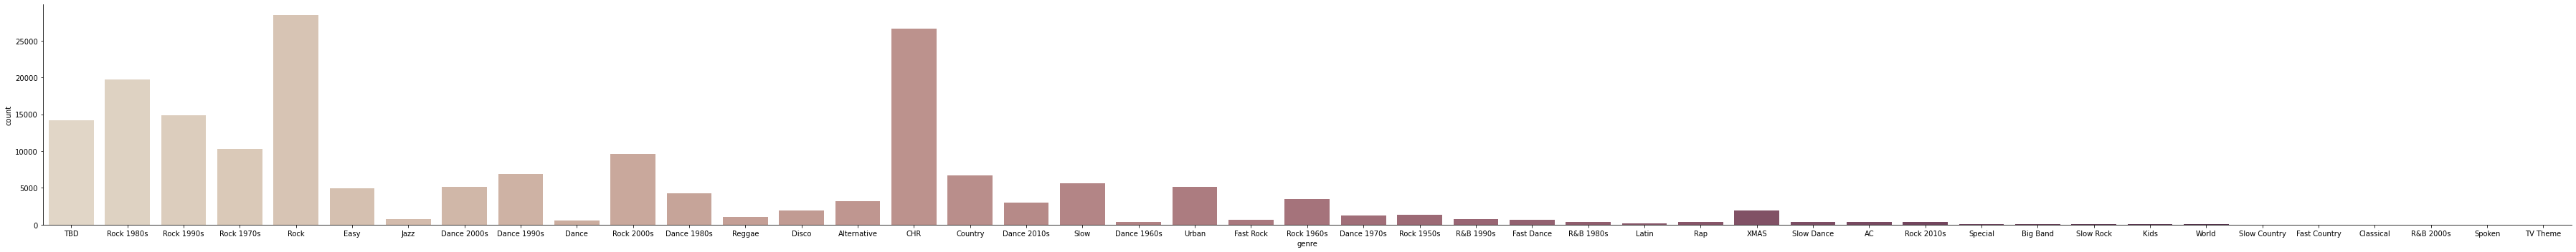
\includegraphics[scale=0.15]{genre_count.png}
\caption{Genre vs its count}
\label{fig:jobInformationDialog}
\end{figure*}

\begin{figure*}[here]
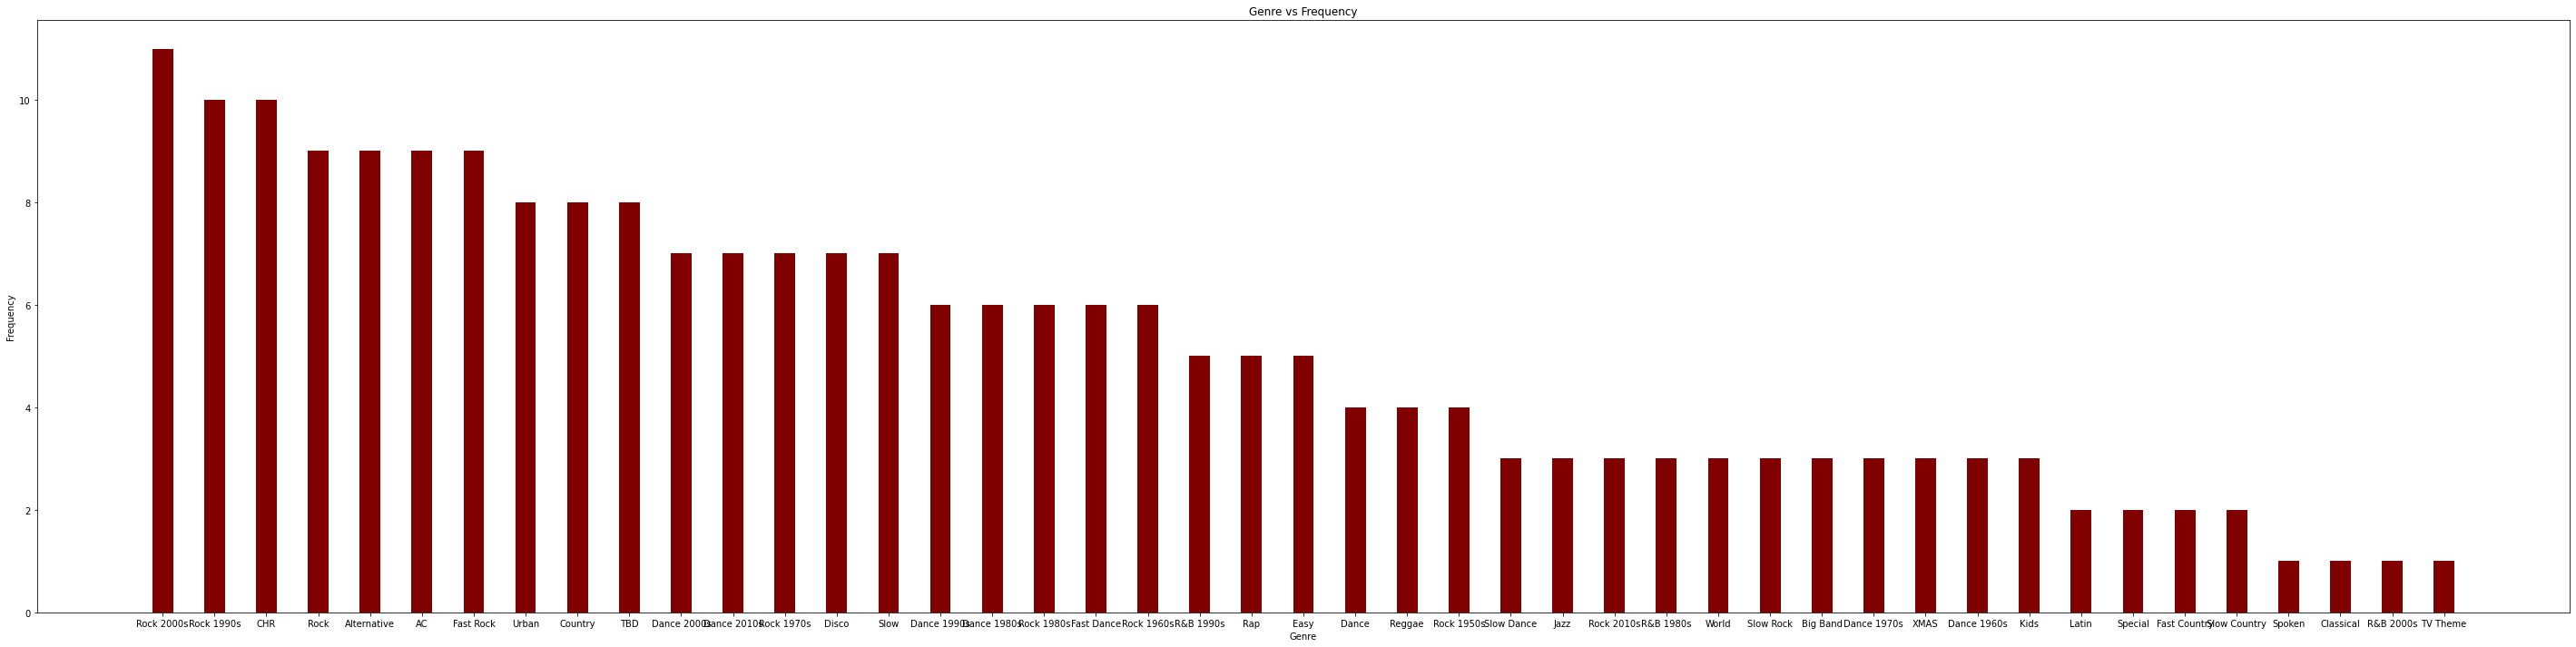
\includegraphics[scale=0.17]{index.png}
\caption{Genre vs its frequency}
\label{fig:jobInformationDialog}
\end{figure*}

Not to worry, the images will be placed in a folder and can be viewed separately.
After that is done, the rows that have NA or empty results (no genres were matched) were dropped, viewing this was easy - using a tool in python made it quick to detect null values. It is hard to visualize the data set and their relations to each other, especially in a clustering model; however viewing their frequencies in the data set may prove that many people like the same music, and some people have the same taste. This is proven true after seeing the counts of songs based on their frequencies in the genre.

The features being represented in this data set are mainly using strings and none of them use integers or numerical data, these strings can be directly converted into numerical data using sklearn. However, in one of the functions provided in the ipynb file, it can be noted that the function automatically changes them into integers or created a dictionary to know in which row in the data set they exist in.


\subsection{Software}
 
 For preprocessing of the dataset and the creation of the previously mentioned models, different software has been used such as Jupyter Notebook, Excel, Visual Studio Code, Overleaf, and Google Co-lab for fast computation. Moreover, the following Python libraries were used: Pandas, NumPy, Matplotlib, requests, BeautifulSoup, scikit-learn, scipy and LightFm \cite{kula_2016}. 

 As for how was the work coordinated, most of the work is updated on WhatsApp, with a weekly meeting on Google Meet. Links to the Overleaf document as well as links to Word documents were shared.
 
\subsection{Hardware}
The work is mainly done on a laptop and some were
done on a Mac mini with an M1 processor for faster
ML processing. However, there were some calculation-intensive calculations that required a dedicated
graphics card. In this case, after using a laptop (Laptop 1) with both an intel i7-9750H and an Nvidia GTX 1650
to run the algorithm’s intense operation this process took around three hours to match the dataset of the University of Waterloo with the 12 million row dataset, which is an intensive process, in good faith to not repeat the process again, the output file is saved into a CSV file. Each method is done on a different machine, Method one was done on Laptop 1, while Methods 2 and 3 were done on Laptop 2 (Omar's Laptop) using Google Colab. Later on, more resource intense applications were done on Colab, for it provides exactly 15 GBs of dedicated RAM instead of the 12 GBs of RAM on laptops where 4GBs were taken due to opening other applications, as well as background applications.

\section{Results and Discussion}


After fitting the data into the model, it is divided into a train\_test\_split array, where the Area Under the Curve and Precision is calculated, and the AUC being used is sklearn.metrics.auc(x, y).mean() which is a method used to compute the Area Under the Curve, it is "the measure of the ability of a classifier to distinguish between classes" \cite{bhandari_2022}. It is hard to tell if the model in fact did a good job when it came to learning the data set to recommend for users a song; there indeed does exist an output of a song in method 1, but it is hard to tell if the user will like it or not. The precision does not tell as well if the user will like it or not. After inserting a custom user to the data set, at least with Method 1, it seems that it is producing a good recommendation for songs that contributor to Method 1 listens to. 

The weakness of this approach is that it is hard to tell if the model is clustering the information in an unsupervised machine learning model. 

The results from Model 1 are AUC: (train: 0.9716839, test: 0.97279567),
and Precision@K (k=5): (train: 0.40, test: 0.22). The
second method (models 2 and 3) does not use frequency. 
Model 2 gives AUC: (train: 0.99326223, test: 0.9158364), and Precision@K (k=5): (train: 0.6124809,
test: 0.044162657). On the other hand, model 3 gave the following results: AUC: (train: 0.976131, test: 0.9232743), and Precision@K (k=5): (train: 0.388438, test: 0.06182772).
These results can be seen in table 1.

As for the discussion, the accuracy test does not show exactly if the user is being recommended the right song per se. There exists at least one thousand different unique users in this data set, and around nine thousand unique songs as well. For the data set to have more than 0.5 precision at k=5 is to exist two users with both having at least one common song. In retrospect, it is to have one thousand different users who all have at least listened to half of the unique songs that exist in the data set, this is true after understanding the role of the interaction matrix in creating a matrix of users who listen to similar songs with similar features. An example to explain this: let us say Omar and Miguel both listen to Elvis Presley, this would make the model 100\% precise; however, Miguel listens to MGMT as well, this would reduce the precision to about 75\% ±0.5\% just because Miguel listens to another artist. For the model to recommend a song, users should have at least one similar artist, the more similarities one user has to another in the data set, the more precise the predictions are going to be. The problem arises in this context, there are one thousand different users with one user listening to at most 92 unique songs, it is hard to recommend for this user a song since they are "sparse" (there does not exist another who listens to 92 different songs as well).


%Below to show you how to format a table:
\begin{table}
\begin{center}
\begin{tabular}{|l|c|c|} %if you need more columns, just add |
\hline
Method & AUC & Precision at k=5\\ %the & is like a tab where you split the columns
% the \\ means an enter to go to another line
\hline\hline  %hline is to draw a line
Method 1 & $97 &22\pm 0$ \% \\
Method 2 & $91 &4.4\pm 0$ \% \\  %notice how to write a %
Method 3 & $92 &6.1\pm 0$ \% \\  %notice how to write a %
\hline
\end{tabular}
\end{center}
\label{tab:some-table}
\caption{AUC and precision at k=5 test results}
\end{table}

For method one, this interaction matrix is a pure collaborative filtering matrix that is created with help from the frequency being generated using a group\_by method in python. Pure collaborative filtering only takes into account the user\_id and artist\_id into account when creating an interaction matrix, later inhibiting the actual accuracy of the song being recommended. This is where a genre column would be useful. 

On the other hand, methods two and three performed worse than method 1. Method 2 used a pure CF model and took only user\_ids and track\_ids into consideration, while method 3 uses a hybrid approach combining CF and content-based filtering and additionally taking track names, artist names and genres into consideration. Notably, the only main thing that was different was the frequency column between method 1 and the other methods. One may ask: "How does a frequency column create such a jump in the precision at k?" To answer that, the model will understand the most frequent song in each user as explained above (1000 users 4500 songs in common (9000/2)), the frequency allowed the model to understand that the most frequent song was for example: "Electric Feel by MGMT with 490 occurrences". This aided the recommending time, but negatively affected the model creation time, especially when the data is in both String and integers, which is computationally costly. However, incorporating features of the song like in method three in addition to the frequency in method one could lead to recommending songs better than method one because of taking into account the genre column added as well as the other rows (Artist name, track name).

\section{Conclusions}

In conclusion, it is hard to create a music recommender system as the results show even if there are people who understand how music works; the vast amount of data that exists in music as well as the uniqueness of every user makes it extraordinarily hard to recommend them a song to listen to. This is aided by the fact that one user could be listening to ten different genres all at once, which is mind-boggling and tanks the precision of the model. Maybe one model can perform better if it understands the user in a deep manner rather than understanding a set of users. If a model can understand the user and the song's qualities, then it may increase the precision of the model. However, as mentioned before, it is hard to tell if the methods are doing a good job at recommending a song beyond metrics like AUC and Precision@K, there simply does not exist labeled data to compare to, and must be assessed manually by users. This is exactly why Spotify recommends a playlist of songs so that a user can nitpick their favorites of the recommended playlist so the model can understand the user in a more deep manner. 

The authors believe that making the model interactive is the way to go since it increases the likelihood of it producing accurate results. In this case, it would be the user adding the song to his/her playlist or adding the song to the liked song category. Another suggestion for future work would be to apply a hybrid model instead of a pure CF model in method 1 that frequency into consideration as mentioned before. Furthermore, more features and data could be useful to build a more precise model.

\section{Contributions}

As for the contribution, Miguel worked with Omar together on creating the 150kGenres.csv dataset by downloading the 12 million row data set from Kaggle and using Google Meet as a platform to collaborate on how to do web scraping and linking the two data sets together. Omar found the online database \cite{tompkins_n.d.} for the genres and worked on the web scraping code and Miguel ran that code on his hardware.

Miguel Ibrahim worked on Method 1 which included a pure LightFM collaborative filtering model that accesses the frequency of songs to better understand what people like, as well as recommending one song to a pre-existing user in the data set. Before using the data set called 150kGenres.csv, the data needs to be cleaned by removing null values (if any) and dropping the Unnamed row: 0. After adding a frequency row using the group by function, the data can be split into artist\_dictionary and user\_dictionary. The artist dictionary consists of the artist's name and its location of it in the data set. This is later reset to start at 1 instead of a random value that pre-existed in the data set. As for the user\_dictionary, it consists of the unique user\_ids in the dataset and their positions as well, a similar method is used for user\_ids as well.

Omar Majzoub found an article \cite{mingzhi_2021} that included code for using a dataset to build an interaction matrix and item features that can be used to build a LightFM model as well as code to create a pure CF model and a hybrid model both with LightFM. The code was altered to fit the dataset of this paper placing tracks as our "products" that users interacted with.

The authors both worked on this report.

%the section below is to include the references
{\small
\bibliographystyle{ieee}
\bibliography{references}
}

\end{document}
